\documentclass[a4paper]{../birkjour}

\usepackage{../fouche-copy}
\makeatletter
\def\@settitle{\begin{center}%
  \baselineskip14\p@\relax
  \bfseries
  \uppercasenonmath\@title
  \@title
  \ifx\@subtitle\@empty\else
     \\[1ex]\uppercasenonmath\@subtitle
     \footnotesize\mdseries\@subtitle
  \fi
  \end{center}%
}
\def\subtitle#1{\gdef\@subtitle{#1}}
\def\@subtitle{}
\makeatother

\newcommand{\var}[3][]{
  \left[\begin{smallmatrix} #2 \\
  #1\downarrow \\ #3
  \end{smallmatrix}\right]}
\newcommand{\cvar}[3]{
  \begin{xsmallmatrix}{0em}
  & #1 \\ #2 & \downarrow \\ & #3
  \end{xsmallmatrix}}

\def\la{\langle}
\def\ra{\rangle}
\def\lr#1#2{\la #1,#2\ra}
\def\tr{\textsf{t}}
\newcommand{\true}{\texttt{t}}
\def\id{\text{id}}
\author{Dario Dentamaro}
\address{Dario \textsc{Dentamaro}: }
\email{dio@cane.it}
\author{Fosco Loregian}
\address{%
  Fosco \textsc{Loregian}: %
  Tallinn University of Technology, %
  Institute of Cybernetics, Akadeemia tee 15/2,%
  12618 Tallinn, Estonia}
\email{fosco.loregian@taltech.ee}
\email{fosco.loregian@gmail.com}
\title{Categorical ontology I}
\subtitle{Existence}
\usepackage{proof}

\usepackage{minted}
\def\mil#1{\mintinline{haskell}{#1}}
\newcommand{\po}[1][dr]{\save*!/#1+1.5pc/#1:(1,-1)@^{|-}\restore}
\newcommand{\pb}[1][dr]{\save*!/#1-1.5pc/#1:(-1,1)@^{|-}\restore}


\setlength{\epigraphwidth}{.6\textwidth}
\setcounter{tocdepth}{1}

\usepackage{fontawesome}
\title{Categorical Ontology I$\frac{1}{2}$: Functorial erkennen}
%== authors' info
% \author{Blinded authors}
%
%
%
\author{Dario \textsc{Dentamaro}}
\address{Università degli Studi di Firenze,\newline Dipartimento di Matematica e Informatica
        }
\email{dario.dentamaro@stud.unifi.it}
% \email{dariodentamaro26@gmail.com}
%
\author{Fosco \textsc{Loregian}}
\address{ Tallinn University of Technology,\newline %
          Institute of Cybernetics, Akadeemia tee 15/2, \newline %
          12618 Tallinn, Estonia }
\email{fosco.loregian@taltech.ee}
% \email{fosco.loregian@gmail.com}


\usepackage{booktabs}
% \usepackage{braket}
%== `braket' confligge con alcune macro già esistenti 
\newcommand{\bk}[1]{\langle #1\rangle}
\begin{document}

\maketitle
\tableofcontents

\section{Introduction}
Qui spiegare il senso del lavoro: fornire gli strumenti per una semantica funtoriale delle teorie, che non siano solo scientifiche. Il lavoro si inserisce parzialmente nel nostro tentativo di fornire strumenti matematici adeguati per trattare problemi di natura filosofica. In questo caso si prende una delle parti meglio sviluppate della filosofia della scienza e la si adegua anche a teorie metafisiche o ontologiche, in più migliorando l'approccio agli oggetti di cui normalmente ci si occupa in questo campo (teorie fisiche e biologiche). Partirei con frase a effetto sul problema del rapporto tra teoria e mondo.

What about 

\epigraph{Life is the life of the world to come, which a man earns by means of the letters.}{Sefer Ozar Eden Ganuz}

\section{Semantical conception of theories}
During the XXth century it was considered necessary to develop a formal treatment of scientific theories. The Wiener Kreis verificationist paradigm/account, and the Neurath theory of `protocollar statements', was the input to elaborate a completely semantical framework for working with scientific theories, and the clue of a pan-linguistic vision of philosophy of science. 

For the sake of strictness the formal account in which Carnap and associates provide their notion of `theory' is known in literature as \emph{syntactical conception of theories} \cite{.} while the introduction of term `semantic' is due to later developments. But the field of epistemology that the logical neopositivism started one can call `semantics of theories', because some characteristics, and above all the underlying ideology, are the same from Carnap to Beth to Suppes, up to the recent canonical uses of physical handbooks. 

[scrivere quali sono queste caratteristiche]

[sintesi delle varie concezioni; le teorie come classi di modelli $\clK$; 
le teorie come oggetti formali]

semantica non standard per teorie empiriche in cui le teorie sono sistemi formali e tutte le nozioni diventano oggetti matematici; più propriamente una \emph{teoria} diventa una struttura $(F_\clL, \clK)$ dove $F_\clL$ è il vero sistema formale e $\clK$ è la classe di tutti i suoi modelli. La nostra strategia è separare ulteriormente $F_\clL$ in due `vocabolari' (per noi, le categorie sintattiche di teorie al primo ordine), uno $P_{F_\clL}$ che rappresenta i termini puri (nel senso di Plantinga) e uno $A_{F_\clL}$ che rappresenta i termini \emph{applicati}. Ergo una teoria $\mathbf{T}$ sarà una particolare tripla $\bk{(P_{F_\clL},A_{F_\clL}), \clK}$ in cui la prima coppia configura una logica (uno `spazio degli stati' che configura una logica). 

La coppia $(P_{F_\clL},A_{F_\clL})$ è poi soggetta a una ulteriore condizione di ammissibilità, cf. \ref{}, chiedendo che esista un profuntore tra le due categorie sintattiche $P_{F_\clL},A_{F_\clL}$.

La specificazione del dominio di $A_{F_\clL}$ determina il tipo di teoria che stiamo considerando (scientifica, strettamente empirica, logico-matematica, metafisica).

Dire che $A_{F_\clL}$ determina le \emph{tipizzazioni} della teoria significa 
dire che svolge lo stesso ruolo della legge $\beta$ nella semantica dello spazio degli 
stati, mentre la classe $\clK$ è isomorfa all'insieme $\mathcal{M}$ dello spazio 
degli stati. Il tipo di $\beta$ determina il tipo di $\mathcal{M}$ che determina il 
tipo di $\mathbf{T} = (\mathcal{M}, \beta)$. Idem nel nostro approccio: $A_{F_\clL} 
= \{\alpha_1,\dots,\alpha_n\}$ determina il tipo, che implementa una logica che determina 
la classe $\clK$. 
%si può generalizzare tutto ciò dicendo appunto che a seconda di come è strutturata la classe $A_{\mathcal{F_L}}$ noi possiamo distinguere le teorie anche al di fuori dell'ambito strettamente scientifico. Questa considerazione va a scomparire proprio con ciò che emerge in sezione 6: eliminando questa distinzione ottieni un account più generale di trattamento delle teorie%

\subsection{The Two Dictionaries}
Nella concezione neopositivistica la distinzione tra legge teorica e legge empirica non è dovuta alla natura ipotetica della prima (anche una legge empirica può esserlo) quanto dal fatto che i due tipi di legge contengono tipi differenti di termini \cite{}. La distinzione è quindi formale, e indica una approccio prettamente linguistico a questioni epistemologiche. 

Anche in questa visione `sintattica' \cite{ } una teoria è sempre una struttura che contiene un sistema formale $\mathcal{F_L}$ e la classe $\clK$ dei suoi modelli. La strategia carnapiana per rendere conto della presenza di entità `osservazionali' e quindi, a rigore, non formalizzabili, all'interno di teorie scientifiche è quella di considerare due diversi dizionari: $\mathcal{V_T}$ che contiene \emph{termini teorici} e $\mathcal{V_O}$ che contiene \emph{termini osservativi}. Intuitivamente $\mathcal{F_L} = \mathcal{V_T} \cup \mathcal{V_O}$, ma piu precisamente $\mathcal{F_L} = \mathcal{V_T} \uplus_\varphi \mathcal{V_O}$.

Per derivare una legge empirica da una teorica Carnap introduce delle \emph{correspondance rules} ma senza definirle adeguatamente. Possiamo analogamente fornire il framework `viennese' di una \emph{funzione di traduzione} $\varphi: \mathcal{V_O} \to \mathcal{V_T}$ tale che ogni termine osservativo $\omega_j$ viene sostituito da un corrispondente teorico $\varphi (\omega_j)$ \footnote{In generale Carnap sembra assumere che $\mathcal{V_O} \subset \mathcal{V_T}$ ma specifica comunque che è errato dire che gli O-terms siano esempi di T-terms.}.
%qui va aggiunta la funzione di "applicazione" $\psi: \mathcal{V_T} \to \mathcal{V_O}$ che fa il percorso inverso di quella di traduzione. è un modo migliore per rappresentare il dibattito di inizio 900: quale delle due funziona meglio? Non esiste la risposta corretta (per i neopositivisti presumibilmente la Ramsey version della def 2.1 coinvolge $\psi$ e ha come oggetti elementi di $\mathcal{V_O}$). La risposta storicamente più accurata è "entrambe alternativamente". Bene, altra cosa risolta dalla sezione 6% 

\begin{definition} [Wiener Definition]
	Una teoria $\mathbf{T}$ è una coppia $\bk{\tau_i, \varphi (\omega_j)}$ dove $\tau_i \in \mathcal{V_T}$ e $\omega_j \in \mathcal{V_O}$
\end{definition}



[\cite{} Carnap da pag. 299; importante la 314]

\subsection{\emph{Was Sind und was sollen die Erkennen?}}

La strategia carnapiana è figlia della distinzione di Moritz Schlick \cite{.} tra \emph{kennen} e \emph{erkennen} ... [spiegare la manfrina e la nostra `traduzione']

In questo paragrafo parlerei della questione `sì ma cosa sono gli `osservativi' nella nostra semantica funtoriale?', dell'arbitrarietà della divisione in due categorie sintattiche, per comodità nel trattamento di determinate teorie, e introdurrei alla tensione tra teorico e osservazionale che si sviluppa formalmente in seguito (cenno storico in nota al perchè i neopositivisti fanno la ramseyfication e perchè a noi non interessa (citare lo Weinberg)).  
%forse tutta sta parte confluisce in section 6%

\section{Profunctors / Grothendieck construction}
\label{sec:org7dd09e1}
Ci sono due competing pictures che descivono una relazione $R$ che sussiste tra due insiemi $A,B$
\begin{enumtag}{r}
\item \label{r_1} a relation $R$ is a subset of the cartesian product $A\times B$;
\item \label{r_2} a relation $R$ is a function $A\times B \to \{0,1\}$.
\end{enumtag}
Note that the notion of `relation between $A$ and $B$' is inherently symmetric, in the sense that such $R$ can be regarded both as a relation `from' $A$ `to' $B$, and as a relation `from' $B$ `to' $A$.

The second important preliminary remark is that every relation $R$ between sets $A,B$ gives rise to a \emph{Galois connection} 
\[R^* :PA \leftrightarrows PB : R_* \label{adjunzia} \]
between the powersets $PA=2^A$ and $PB = 2^B$: the set $U\subset A$ goes to the set $R^*U$ of all $b$ such that $(a,b)\in R$ for all $a\in U$; in an exactly symmetric way, a set $V\subseteq B$ goes to the set $R_*V = \{a\in A\mid (a,b) \in R,\, \forall b\in V\}$.

From here, using a process known as `categorification' \cite{baez_catego}, we can replace a two-valued relation $R\subseteq A\times B$ with a \emph{set-valued} functor $\clA^\op\times\clB \to \Set$ between two (small) categories $\clA,\clB$.\footnote{The reason why the category $\clA$ is twisted with an `$^\op$' functor is that we want to bestow the hom functor $\hom_{\clA} : \clA^\op\times\clA \to \Set$ with the r\^ole of identity arrow; in the categorification perspective, hom plays the r\^ole of the diagonal relation $R=\Delta : A\to A\times A$.} More precisely, we can give the following definition.
\begin{definition}[Profunctor]\label{def_profu}
  
\end{definition}
The intuition behind \autoref{def_profu} is that $\fkR(A,B)$ is the \emph{type} whose terms are all proofs che tra $(A,B)\in\clA^\op\times\clB$ sussiste la `relazione generalizzata' $\fkR$. This intuition agrees with the fact that when instead of $\Set$ a profunctor $\fkR$ takes values in the 0-dimensional category $\{0\le 1\}$, then the type of proofs that $R(A,B)$ is a yes/no kind of space.

From here, one can build a rich and expressive theory; we are contempt with a careful analysis of the analogue of \ref{r_2} and \eqref{adjunzia} above: the latter is the scope of \autoref{sec:org1a423df}, we now concentrate on describing an ubiquitary technical tool in category theory.
\subsection{Grothendieck construction}
The Grothendieck construction is the tool allowing to formalise the equivalence between a relation understood as a function $R : A\times B \to \{0,1\}$, and a subset $R\subseteq A\times B$, when `relation' is understood in the sense of \autoref{def_profu} above, i.e. a profunctor $\fkR : \clA \pto \clB$. Each such $\fkR$ can be realised as a suitable `fibration' $p_\fkR : \clE \to \clA^\op\times\clB$, that in turn uniquely determines $\fkR$.
We now recall a few basic definitions.
\begin{definition}\label{eltsf}
	Let $\clC$ be an ordinary category, and let $W : \clC\to \Set$ be a functor; the \emph{category of elements} $\elts{\clC}{W}$ of $W$ is the category which results from the pullback
  \[
    \xymatrix{
      \elts{\clC}{W}\ar[r]\ar[d] \pb & \Set_* \ar[d]^U \\
      \clC \ar[r]_W & \Set
    }
  \]
  where $U : \Set_*\to\Set$ is the forgetful functor which sends a pointed set to its underlying set.
  
  More explicitly, $\elts{\clC}{W}$ has objects the pairs $(C\in\clC, u\in WC)$, and morphisms $(C,u)\to (C',v)$ those $f\in \clC(C,C')$ such that $W(f)(u)=v$.
\end{definition}
\begin{definition}[Discrete fibration]
	\label{def:dfib}
	A \emph{discrete fibration} of categories is a functor $G : \clE \to \clC$ with the property that for every object $E\in\clE$ and every arrow $p : C\to GE$ in $\clC$ there is a unique $q : E'\to E$ `over $p$', i.e. such that $Gq=p$.
\end{definition}
Taking as morphisms between discrete fibrations the morphisms in $\Qat/\clC$, we can define the category $\DFib(\clC)$ of discrete fibrations \emph{over} $\clC$.
\begin{proposition}\label{fibelem}
	The category of elements $\elts{\clC}{W}$ of a functor $W : \clC\to \Set$ comes equipped with a canonical \emph{discrete fibration} to the domain of $W$, which we denote $\Sigma : \elts{\clC}{W}\to \clC$, defined forgetting the distinguished element $u\in Wc$.
\end{proposition}
With this terminology at hand, we can consider the \emph{category of elements} \ref{eltsf} of a functor $F : \clC\to \Set$; this sets up a functor from $\Qat(\clC,\Set)$ to the category of discrete fibrations over $\clC$: the Grothendieck construction asserts that this is an equivalence of categories.%, as defined in \ref{def:equcat}.
\begin{theorem}\label{thm:equconfib}
	There is an equivalence of categories
	\[
		\Qat(\clC^\op,\Set) \to \DFib(\clC)
	\]
	defined by the correspondence sending $F\in\Qat(\clC,\Set)$ to its \emph{fibration of elements}  $\Sigma_F : \elts{\clC}{F} \to \clC$.
\end{theorem}
The inverse correspondence sends a discrete fibration $\Phi : \clE \to \clC$ to the functor whose action on objects and morphisms is depicted in the following image:
\begin{center}
  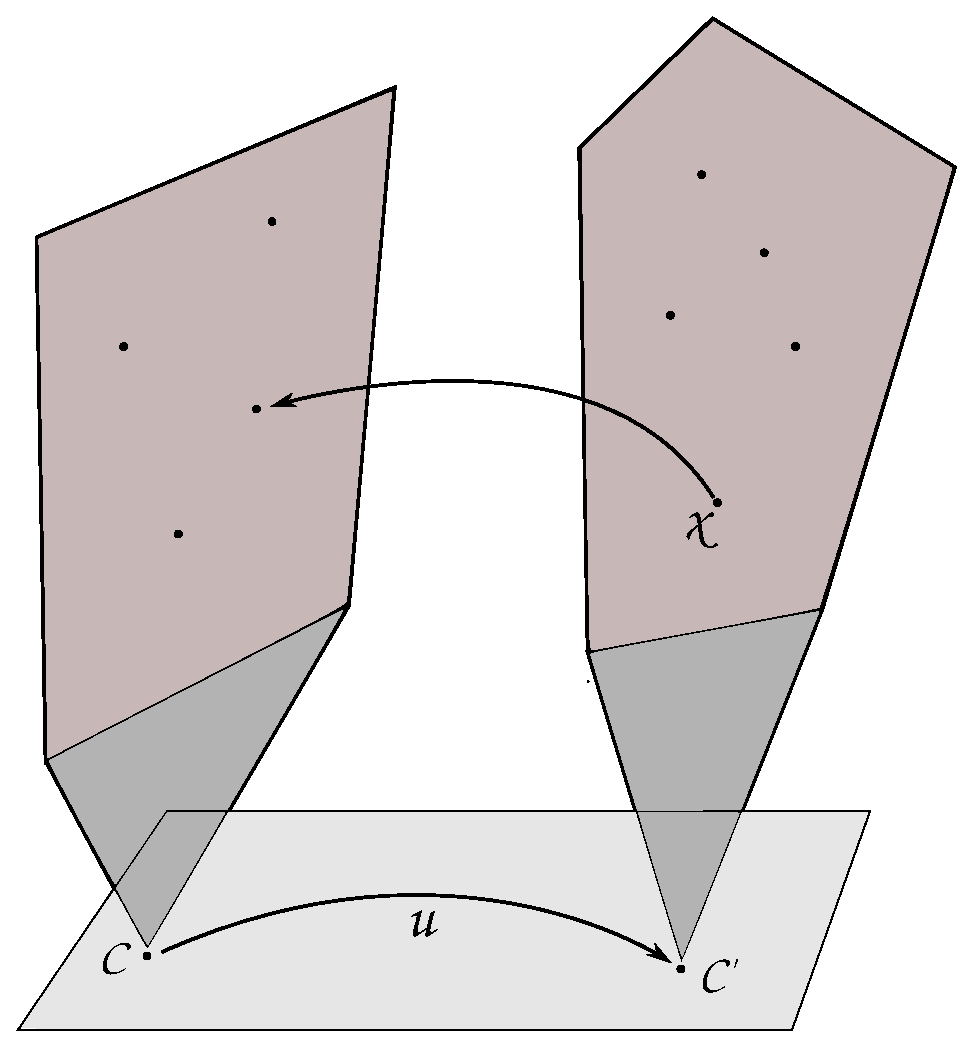
\includegraphics[width=.325\textwidth]{disegno.eps}
\end{center}
\begin{corollary}
  Given a profunctor $\fkR : \clA \pto \clB$, regarded as a functor $R : \clA^\op\times \clB \to \Set$, we can consider the category of elements $\elts{\clA^\op\times\clB}{R}$; this is often called the \emph{collage} or the \emph{graph} of $R$.
\end{corollary}
\section{Nerve and realisations}
\label{sec:org1a423df}
We start by recalling the universal property of the category of presheaves over $\clC$:
let $\clC$ be a small category, $\clW$ a cocomplete category; then, precomposition with the Yoneda embedding $\yon_{\clC} : \clC \to [\clC^\op, \Set]$ determines a functor
\[\Qat([\clC^\op, \Set], \clW)\xto{\firstblank\circ \yon_{\clC}} \Qat(\clC,\clW),\]
that restricts a functor $G : [\clC^\op, \Set]\to \clW$ to act only on representable functors, confused with objects of $\clC$, thanks to the fact that $\yon_\clC$ is fully faithful. We then have that
\begin{theorem}\label{yext_are_good}\leavevmode
	\begin{enumtag}{ye}
		\item The universal property of the category $[\clC^\op, \Set]$ amounts to the existence of a left adjoint $\Lan_{\yon_{\clC}}$ to precomposition, that has invertible unit (so, the left adjoint is fully faithful).
	\end{enumtag}
	This means that $\Qat(\clC,\clW)$ is a full subcategory of $\Qat([\clC^\op, \Set], \clW)$. Moreover
	\begin{enumtag}{yi}
		\item The essential image of $\Lan_{\yon_{\clC}}$ consists of those $F : [\clC^\op, \Set] \to \clW$ that preserve all colimits.
		\item If $\clW = [\clE^\op, \Set]$, this essential image is equivalent to the subcategory of left adjoints $F : [\clC^\op, \Set] \to [\clE^\op, \Set]$.
	\end{enumtag}
\end{theorem}
As a consequence of this,
\begin{definition}[Nerve and realisation contexts]\label{nr_para}\index{Nerve!--- context}
	Any functor $F : \clC\to \clW$ from a small category $\clC$ to a (locally small) \emph{cocomplete} category $\clW$ is called a \emph{nerve\hyp{}realisation context} (a NR \emph{context} for short).
\end{definition}
Given a NR context $F$, we can prove the following result:
\begin{proposition}[Nerve-realisation paradigm]\label{nervereal}
	The left Kan extension of $F$ along the Yoneda embedding $\yon_\clC : \clC\to [\clC^\op, \Set]$, i.e. the functor
	\[L_F=\Lan_{\yon_\clC} F : [\clC^\op, \Set]\to \clW\]
	is a left adjoint, $L_F\dashv N_F$. $L_F$ is called the $\clW$-\emph{realisation functor} or the \emph{Yoneda extension} of $F$, and its right adjoint the $\clW$-\emph{coherent nerve}.
\end{proposition}
\begin{proof}
	From a straightforward computation, it follows that if we define $N_F(D)$ to be $C\mapsto \clW(F C,D)$, this last set becomes canonically isomorphic to $[\clC^\op,\Set](P,N_F(D))$. We can thus denote $\clW(F,1)$ the functor $N_F : D\mapsto \lambda C.\clW(F C,D)$.
\end{proof}
Now, let's review the way in which a profunctorial analogue of \eqref{adjunzia} can be obtained: \autoref{nervereal} yields that a functor 
\[ \fkR : \clA^\op\times \clB \to \Set \]
whose mate under the adjunction $\Qat(\clA^\op\times \clB ,\Set)\cong\Qat(\clB,[\clA^\op,\Set])$ is a functor 
\[ \hat R : \clB \to \Qat(\clA^\op,\Set) \]
determines a NR paradigm, and thus gives rise to a pair of adjoint functor 
\[ \Lan_{\yon_\clB} \hat R : \Qat(\clB^\op,\Set) \leftrightarrows \Qat(\clA^\op,\Set) : [\clA^\op,\Set](\hat R,1). \]
We have just proved 
\begin{proposition}\label{equ_prof_cocont}
  There is an equivalence of categories between $\Prof(\clA,\clB)$ and the category of colimit preserving functors $\Qat(\clB^\op,\Set) \to \Qat(\clA^\op,\Set)$.
\end{proposition}
\section{Theories and models}
\label{sec:orge02f333}
In this section we exploit the terminology established before.
\begin{definition}[Theory]\label{teoria}
  A \emph{theory} $\clL$ is the syntactic category $\clT_L$ (cf. \cite{lambek1988introduction}) of a first-order, finitely axiomatisable language $L$.
\end{definition}
\begin{definition}[World, Yaldabaoth]\label{mondo_yalda}
  A \emph{world} is a large category $\clW$; a \emph{Yaldabaoth} is a world that, as a category, admits all small colimits.\footnote{Also known as \emph{Yaltabaoth} or \emph{Ialdabaoth}, \dots}
\end{definition}
Given a theory $\clL$ and a world $\clW$, a $\clL$-\emph{canvas} of $\clW$ is a functor 
\[\xymatrix{\clL \ar[r]^\phi & \clW.}\]

A canvas $\phi : \clL \to \clW$ is a \emph{\science} if $\phi$ is a dense functor.
\begin{remark}
  The NR paradigm exposed in \autoref{nr_para} now entails that given a canvas $\phi : \clL \to \clW$
  \begin{itemize}
    \item If $\clW$ is a world, we obtain a \emph{representation} functor 
    \[ \xymatrix{\clW \ar[r] & [\clL^\op, \Set];} \]
    this means: given a canvas $\phi$ of the world, the latter leaves an image on the canvas.
    \item If in addition $\clW$ is a Yaldabaoth, we obtain a NR-adjunction
    \[\xymatrix{\clW \ar@<3pt>[r] & \ar@<3pt>[l] [\clL^\op, \Set];}\]
    this has to be interpreted as: if $\clW$ is sufficiently expressive, then models of the theory that explains $\clW$ through $\phi$ can be used to acquire a two-way knowledge. Phenomena have a theoretical counterpart in $[\clL^\op,\Set]$ via the nerve; theoretical objects strive to describe phenomena via their realisation.
    \item If an $\clL$-canvas $\phi : \clL \to \clW$ is a \science, `the world' is a full subcategory of the class of all modes in which `language' can create interpretation.
  \end{itemize}
\end{remark}
The terminology is chosen to inspire the following idea in the reader: science strives to define \emph{theories} that allow for the creation of world representations; said representations are descriptive when there is dialectic opposition between world and models; when such representation is faithful, we have reduced `the world' to a piece of the models created to represent it.

The tongue-in-cheek here is, a science (in the usual sense of the world) can never attain the status of a \science, if not potentially; attempts to generate scientific knowledge are the attempts of
\begin{itemize}
  \item recognizing the world $\clW$ as a sufficiently expressive object for it to contain phenomena and information;
  \item carve a language $L$, if necessary from a small subset of $\clC$, that is sufficiently `compact', but also sufficiently expressive for its syntactic category to admit a representation into the world;
  \item obtaining an \emph{adjunction} between $\clW$ and models of the worlds obtained as models of the syntactic theory $\clL$; this is meant to generate models starting from observed phenomena, and to predict new phenomena starting from models;
  \item obtaining that `language is a dense subset of the world', by this meaning that the adjunction outlined above is sufficiently well-behaved to describethe world as a fragment of the semantic interpretations obtained from~$\clL$.
\end{itemize}
It is evident that there is a tension between two opposite feature that $\clL$ must exhibit; it has to be not too large to remain tractable, but on the other hand it must be large enough in order to be able to speak about `everything' it aims to describe.

Regarding our definition of \science, we can't help but admit we had this definition in mind \cite[2.1]{biologia}:
\begin{definition}[\protect{\cite[2.1]{biologia}}]
  A \emph{scientific theory} $\clT$ consists of a formal structure $F$ and a class of interpretations $M_i$, shortly denoted as $\clT=\langle F,M_i\mid i\in I\rangle$. The structure $F$ consists on its won right of 
  \begin{itemize}
    \item a language $\clL$, in which it is possible to formulate propositions. If $\clL$ is fully formalised, it will consist of a finite set of symbols, and a finite set of rules to determine which expressions are well-formed. This is commonly called \emph{technical language};
    \item A set $A$ of `axioms' or `postulates' in $\clL^\star$;
    \item A \emph{logical apparatus} $R$, whose elements are rules of inference and logical axioms, allowing to prove propositions.
  \end{itemize}
\end{definition}
The language of category theory allows for a refined rephrasing of the previous definition: we say that a \emph{$\clS$-scientific theory} is the following arrangement of data:
\begin{enumtag}{st}
\item a formal language $\clL$;
\item the syntactic category $T_\clL$, obtained as in \cite{lambek1988introduction};
\item the category of functors $\Qat[T_\clC, \clS]$, whose codomain is a Yaldabaoth.
\end{enumtag}
More than often, our theories will be $\Set$-scientific: in such case we just omit the specification of the semantic Yaldabaoth, and call them \emph{scientfic theories}.

Since the category $\Qat[T_\clC, \Set]$ determines $\clL$ and $T_\clL$ completely, up to Cauchy-completion \cite{borceuso-cauchy}, we can see that the triple $(\clL, T_\clL, \Qat[T_\clL,\Set])$ can uniquely be recovered from its model category $\Qat[T_\clC, \Set]$. We thus comply to the additional abuse of notation to call `scientific theory' the category $\Qat[T_\clL,\Set]$ for some $T_\clL$.

So, a `coherent correspondence linking expressions of $\clF$ with semantic expressions' boils down to a functor; this is compatible with \cite[2.1]{biologia}, and in fact an improvement (the mass of results in category theory become readily available to speak about --scientific-- theories; not to mention that the concept of `formal structure' is never rigorously defined throughout \cite{biologia})
\section{The tension between observational and theoretical}
\label{sec:orge11c3c4}
When working with categorified relations, it is unnatural and somewhat restrictive considerare lo spazio per i valori che la proposizione `$(a,b)\in R$' può assumere come avente solo due valori; instead we would like to consider the entire \emph{space} of values that a proposition can take, or rather the type of proofs that $(a,b)\in R$ is true.

This intuition is based on the proportion
\begin{center}
  truth values : proposition = section : presheaf
\end{center}
In simple terms, categorifying a proposition $P : X\to \{0,1\}$ that can or cannot hold for an element $x$ of a set $X$, we shall marry the constructive church and say that there is an entire \emph{type} $PC$, image of an object $C\in\clC$ under a functor $P : \clC \to \Set$, whose \emph{terms} are the \emph{proofs} that $PC$ holds true. This is nothing but the propositions-as-types philosophy, in (not so much) disguise: \cite{a,b,c}

The important point for us is that the dialectical tension between observational and theoretical can be faithfully represented through profunctor theory; one can think of propositional functions as relations $(x,y)\in R$ iff the pair $x,y$ renders $\phi$ true; we use this idea, suitably adapted to our purpose and categorified. This very natural extension of propositional calculus, pushed to its limit, yields the following reformulation of the `tension between observational and theoretical' of \cite{u,v,w}
\begin{definition}
  Let $\clT,\clO$ be two small categories, dubbed respectively the \emph{theoretical} and the \emph{observational} settings. A \emph{$(1,1)$-ary Ramsey map} is merely a profunctor 
  \[\fkK : \clT^\op \pto \clO\]
  or, spelled out completely, a functor $\fkK : \clT\times \clO \to \Set$.
\end{definition}
Particular $(1,1)$-ary Ramsey maps can be obtained by elementary means:
\begin{example}
 Every functor $F : \clA \to \clB$ gives rise to a profunctor $F_* := \clB(1,F) : \clB^\op\times \clA\to\Set$ and a profunctor $F^* := \clB(F,1) : \clA^\op\times\clB \to \Set$ as in \autoref{nervereal}; the two functors are mutually adjoint, $F^*\dashv F_*$, see \cite{}. This yield an example of what we call \emph{representable} Ramsey maps. \foo{Say more; also, why (1,1)-ary? Wait and see}
\end{example}
\begin{definition}[Observational and theoretical core]
  Let $\fkR : \clT^\op\times \clO \to\Set$ be a Ramsey map, and $\hat R$ the associated canvas. Let 
  \[ \Lan_{\yon_\clO}\hat R : [\clO^\op,\Set] \leftrightarrows [\clT^\op,\Set] : N_{\hat R} \]
  be the adjunction between presheaf categories determined by virtue of \autoref{equ_prof_cocont}. Let us consider the equivalence of categories between the fixpoints of the monad $T = N_{\hat R}\circ\Lan_{\yon_\clO}\hat R$ and the comonad $S=\Lan_{\yon_\clO}\hat R\circ N_{\hat R}$; this is the equivalence between the \emph{observational core} $Fix(T)\subseteq [\clO^\op,\Set]$ and the \emph{theoretical core} $Fix(S)\subseteq [\clT^\op,\Set]$.
\end{definition}
\begin{remark}
Observational core and theoretical core always form equivalent categories; the tension in creating a satisfying image of reality as it is observed oscillates between the desre to enlarge as much as possible the subcategory of $[\clO^\op,\Set]$ with which our theoretical model is equivalent, where we can have access to $\clT, [\clT^\op, \Set]$ only.
\end{remark}
The reader might have observed, now, that there is nothing in their mere syntactical presentation allowing to tell apart the observational and the theoretical category; this can be justified with the fact that the bicategory $\Prof$ of \autoref{def_profu} is endowed with a canonical self-involution, exchanging the r\^ole of domain and codomain of 1-cells, and thus of the theoretical and observational category $\clT,\clO$. 



This might help to solve the conundrum posed by the existence of `fictional objects'. Sherlock Holmes clearly is the object of a theoretical category. Gandhi is the object of an observational category. But as linguistic objects they can't be told apart completely; they can be at most separated by a profunctor embedding the former in a realistic but fictitious model (that is, for example, the Reichenbach falls), and representing the latter as part of a fictional model (for example, as part of a movie directed by R. Attenborough).

The notion of Ramsey map as given above is unnecessarily restrictive, and does not account for many sorts of configurations that can occur in practice:
\begin{itemize}
  \item a single observational token $O$ can't be described by a single theoretical token $T_1$, but instead needs $T_1,\dots,T_r$;
  \item inverting the r\^oles, a single theoretical token describes not only $O$, but different $O_1,\dots,O_s$.
\end{itemize}
Thus we must admit \emph{multiple} arguments for the domain and codomain of a Ramsey map. This yields the notion of a \emph{$(n,m)$-ary Ramsey map}.
\section{Ramseyfication and beyond: generalised profunctors}
\label{sec:org50db6c2}
We can generalise the definition above to encompass Ramsey sentences:
\begin{definition}
  Let $\clT,\clO$ be two categories; a \emph{Ramsey map}, or a \emph{$(n,m)$-ary Ramsey map} is a profunctor $\fkK : \clT^n \pto \clO^m$; note that we allow $n,m$ to be zero; in that case, $\clA^0$ is understood to be the terminal category $\boldsymbol{1}$.
\end{definition}
The intuition behind this definition is as follows: given $\uT\in\clT^n, \uO\in\clO^m$, the set $\fkK(\uT, \uO)$ represents the type of proofs that the observational tuple $\uO$ admits a description in terms of the theoretical tuple $\uT$.

This formalism allows to speak about particular worlds, obtained as presheaf categories over observational $\clO$; if $\clT, \clO$ is a theoretical pair, we can instantiate \autoref{nervereal} above in the particular case where $\clW = [\clO^\op, \Set]$ (observe that in this case $\clW$ is a Yaldabaoth). We can thus address a certain number of questions, arising from the canonical adjunction obtained by virtue of \autoref{equ_prof_cocont}:% and \autoref{}:
\[
  \xymatrix{ [(\clO^m)^\op, \Set] \ar@<3pt>[r] & \ar@<3pt>[l] [(\clT^n)^\op, \Set];}
\]
It is worth to mention that since the diagram
\[
\vcenter{\xymatrix{
  (\clO^m)^\op \ar[rr]\ar[dr]&& [(\clT^n)^\op, \Set] \ar[dl]\\
  & [(\clO^m)^\op, \Set]
}}
\]
is pseudocommutative, the composition $L\circ y$ s equal to (the mate of) $\fkK$. This means: $\clO$-models, when interpreted inside $\clT$-models, carry representations corrisponding to the observational tokens interpreted in $\clT$-models; that is, the representation is coherent over observational tokens, that is\dots
\begin{remark}
  The operation
  \[\exists \uX . \fkK(\uO, \uX)\]
  translates into
  \[\lambda \uO.\fkK(\uO, F\uO)\]
  whenever there is an adjunction $F : \clO \leftrightarrows \clT : G$ between the theoretical and the observable. This, together with the fact that $F\dashv G$ iff $F^*\cong G_*$ iff $G^*\cong F_*$, suggests the following intuition: in presence of a `botched isomorphism' between observational and theoretical, witnessed by the adjunction $(F,G)$, we consider the theoretical trace left by the (image under $F$ of the) observational tokens, so that the dependency of $\fkK$ from $\uT$ is `eliminated' by means of the adjunction.
  
  Clearly, the opposite procedure is possible: the adjunction $(F,G)$ allows to consider the observational trace left by the image of a theoretical token $\uT$ under $G$, so that 
  \[ \exists \uX . \fkK(\uO, \uX) \equiv \lambda \uO.\fkK(G\uT, \uT) \]
\end{remark}
When the pair arity coarity of a 
\begin{remark}
  The presence of a (generalised) Ramsey map
\end{remark}
\section{Concluding remarks}

\subsection{The Dummett-Plantinga problem}
La manfrina su semantica pura e applicata, applicazione concreta del framework, problema delle modalities, trattare semantica applicata (tipo Lewis) come \emph{teoria} nel senso funtoriale evitando ontological committment bla bla bla (qualche riferimento su sta cosa, remember)

\subsection{Naturalizing Epistemology}
cenni alla questione della incommensurabilità delle teorie, sia tesi Duhem-Quine che accezione radicale di Feyerabend, e come questo framework la risolve (creazione di un linguaggio-ter che non è nè quello del "testo" di partenza nè quello del "testo" di arrivo). 
 
\bibliography{../allofthem}{}
\bibliographystyle{amsplain}
\end{document}
